\documentclass{article}

\usepackage{fancyhdr}
\usepackage{amsmath}
\allowdisplaybreaks
\usepackage{amsthm}
\usepackage{amsfonts}
\usepackage{tikz}
\usepackage[plain]{algorithm}
\usepackage{algpseudocode}
\usepackage{enumitem}
\usepackage{tikz}
\usepackage{pgfplots}
\pgfplotsset{compat=1.18}
\usepgfplotslibrary{groupplots}
\usepackage{comment}

\usetikzlibrary{automata,positioning}

%
% Basic Document Settings
%

\topmargin=-0.45in
\evensidemargin=0in
\oddsidemargin=0in
\textwidth=6.5in
\textheight=9.0in
\headsep=0.25in

\linespread{1.1}

\pagestyle{fancy}
\lhead{\hmwkAuthorName}
\chead{} % empty
\rhead{\hmwkHeaderTitle}
\cfoot{\thepage}

\renewcommand\headrulewidth{0.4pt}
\renewcommand\footrulewidth{0pt}

\setlength\parindent{0pt}

%
% Homework Details
%

\newcommand{\hmwkTitle}{Homework 4}
\newcommand{\hmwkDueDate}{Monday, February 2, 2026}
\newcommand{\hmwkClass}{ICMA 216 Calculus IIIA}
\newcommand{\hmwkClassTime}{Section 1}
\newcommand{\hmwkClassInstructor}{Ruth J. Skulkhu}
\newcommand{\hmwkAuthorName}{\textbf{Jiraroj Wiruchpongsanon (6781617)}}
\newcommand{\hmwkHeaderTitle}{ICMA 216 Calculus IIIA: Homework 4}

%
% Title Page
%

\title{
    \vspace{2in}
    \textmd{\textbf{\hmwkClass:\ \hmwkTitle}}\\
    \normalsize\vspace{0.1in}\small{Due\ on\ \hmwkDueDate}\\
    \vspace{0.1in}\large{\textit{\hmwkClassInstructor\ \hmwkClassTime}}
    \vspace{3in}
}

\author{\hmwkAuthorName}
\date{}

\renewcommand{\part}[1]{\textbf{\large Part \Alph{partCounter}}\stepcounter{partCounter}\\}

%
% Helper Commands
%

\newcounter{partCounter}
\newcommand{\solution}{\textbf{\large Solution}}

\newtheorem*{theorem}{Theorem}

\theoremstyle{remark}
\newtheorem*{remark}{Remark}

\begin{document}

\maketitle
\newpage

\section*{Problem 1 (11.5 Parametric Equations of Lines)}
Find the parametric equations for the line that passes through the points $(6, 3, -3)$ and $(4, -3, 0)$.

\medskip
\solution

we find the directional vector from differences between the two points

\[
  \begin{aligned}
  d &= (6, 3, -3) - (4, -3, 0) \\
  &= (2, 6, -3)
  \end{aligned}
\]

then, using the vector equation, the line can be written in a form of

\[
  \begin{aligned}
  L: r &= r_o + tv \\
  &= \langle 6, 3, -3\rangle + t\langle 2, 6, -3\rangle \\
  &= \langle 6 + 2t, 3 + 6t, -3 - 3t\rangle \text{ where } t \in \mathbb{R}
  \end{aligned}
\]

  and we can derive the parametric equation as

\[
  \boxed{
  \begin{aligned}
  L: x &= 6 + 2t, \\
  y &= 3 + 6t, \\
  z &= -3 - 3t \text{ where } t \in \mathbb{R}
  \end{aligned}}
\]

\vspace{1em}
\hrulefill

\section*{Problem 2 (11.5 Parametric Equations of Lines)}
Find the parametric equations for the line that passes through the origin and parallel to the line $x = 2t, y = 1 - t, z = 4 + 3t$.

\medskip
\solution

focus on directional vector of the paralleled line $r = \langle 2t, 1-t,
  4+3t\rangle$, $v = \langle 2, -1, 3\rangle$ --- the terms with a factor of $t$. \\

  since the line passes through the origin, we set $r_0 = \langle 0, 0, 0\rangle$,
  and we can now construct the vector equation of this line as

  \[
  \begin{aligned}
  L: r &= \langle 0, 0, 0\rangle + t\langle 2, -1, 3\rangle \\
  &= \langle 2t, -t, 3t\rangle
  \end{aligned}
  \]

  and that'll be $\boxed{L: x = 2t, y = -t, z = 3t \text{ where } t \in
  \mathbb{R}}$ for the parametric equation.

\vspace{1em}
\hrulefill

\section*{Problem 3 (11.6 Planes)}
Find the point at which the line with parametric equations $x = 2 + 3t$,
$y = -4t, z = 5 + t$ intersects the plane $4x + 5y - 2z = 18$.

\medskip
\solution

intersecting means that there’s point $(x, y, z)$ which satisfy both the line
and the plane; and since the line is already in its parametric expression form,
we can just substitute $x$, $y$ and $z$ into the plane’s equation as
  \[
  \begin{aligned}
  4(2 + 3t) + 5(-4t) - 2(5 + t) = -10t - 2 &= 18 \\
  \end{aligned}
  \]
which gives $t = -2$, now can substitute $t$ in the parametric equation to get
the intersection point as
  \[
  \begin{aligned}
  (2 + 3(-2),\ -4(-2),\ 5 + (-2)) &= (-4,\ 8,\ 3) \\
  &= \boxed{(-4,\ 8,\ 3)}
  \end{aligned}
  \]

\vspace{4em}
\hrulefill

\section*{Problem 4 (11.6 Planes)}
Find the equation of the plane that contains the line $x = 3 + 2t, y = t, z = 8 - t$ and is parallel to the plane $2x + 4y + 8z = 17$.

\medskip
\solution

 for this one, we find the d value on the plane's $ax + by +
  cz = d$ form that satisfy the line's parametric solution ---
  by substitude the x, y and z value into the plane
  \[
  \begin{aligned}
  2(3 + 2t) + 4(t) + 8(8 - t) &= 6 + 4t + 4t + 64 - 8t \\
  &= 70 = d
  \end{aligned}
  \]
  therefore, the plane's equation is \boxed{2x + 4y + 8z = 70}

\vspace{4em}
\hrulefill

\section*{Problem 5 (11.6 Planes)}
Find an equation of the plane that passes through $(-1,4,-3)$ and is perpendicular to the line\\
$x = 2 + t, y = -3 + 3t, z = -t$.

\medskip
\solution

  we're given the origin point ($r_0$) of (-1, 4, -3) and
  the normal vector ($\vec n$) is embeded in the given
  perpendicular line of $x = 2 + t, y = -3 + 3t, z = -t$.
  we extract the directional vector from the line as $\langle
  1, 3, -1 \rangle$ --- the terms that's a multiple of t.

  \vspace{1em}
  then, using the plane's equation, the equation of the plane
  is
  \[
  \begin{aligned}
  \vec n \cdot (r - r_0) &= \langle 1, 3, -1 \rangle \cdot
  (\langle x, y, z \rangle - \langle -1, 4, -3 \rangle) \\
  &= \langle 1, 3, -1 \rangle \cdot \langle x + 1, y - 4, z +
  3 \rangle \\
  &= (x + 1) + 3(y - 4) - (z + 3) \\
  &= x + 3y - z - 14 = 0
  \end{aligned}
  \]
  \[
  \boxed{x + 3y - z = 14}
  \]

\vspace{4em}
\hrulefill

\section*{Problem 6 (11.6 Planes)}
Find an equation of the plane that passes through the points $P = (1, 3, 2)$,\\
$Q = (3, -1, 6)$ and $R = (5, 2, 0)$.

\medskip
\solution

 compute $\overrightarrow{PQ}$
  \[
  \begin{aligned}
  \overrightarrow{PQ} &= (3,-1,6) - (1,3,2) \\
  &= \langle 2,-4,4 \rangle
  \end{aligned}
  \]

  and $\overrightarrow{PR}$
  \[
  \begin{aligned}
  \overrightarrow{PR} &= (5,2,0) - (1,3,2) \\
  &= \langle 4,-1,-2 \rangle
  \end{aligned}
  \]

  now, we could compute the cross product of the two to get the normal vector as
  \[
  \begin{aligned}
  \vec n &= \overrightarrow{PQ} \times \overrightarrow{PR} \\
  &= \langle 2,-4,4 \rangle \times \langle 4,-1,-2 \rangle \\
  &= \langle 12,20,14 \rangle \\
  &= \langle 6,10,7 \rangle
  \end{aligned}
  \]

  it should look something like this ...

  \begin{center}
  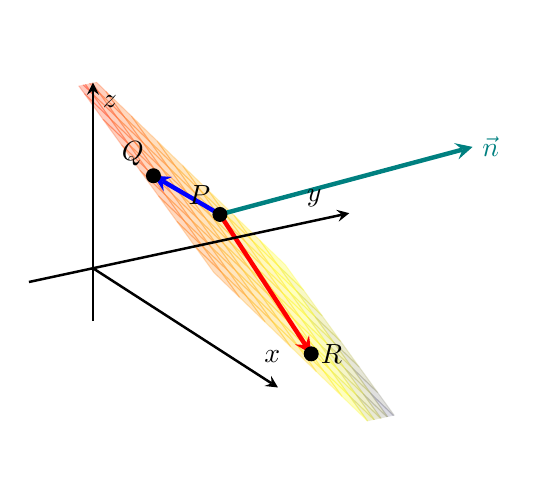
\begin{tikzpicture}
      \begin{axis}[
          width=8cm,
          height=7cm,
          view={60}{30},
          axis lines=center,
          axis line style={line width=0.9pt},
          axis on top,
          ticks=none,
          xlabel={$x$}, ylabel={$y$}, zlabel={$z$},
          xmin=0, xmax=6,
          ymin=-2, ymax=8,
          zmin=-2, zmax=7,
      ]
          \addplot3[
              surf,
              shader=flat,
              opacity=0.25,
              samples=11,
              samples y=11,
              domain=0:6,
              y domain=-2:6,
          ] ({x},{y},{(50 - 6*x - 10*y)/7});

          \addplot3[only marks, mark=*, mark size=2.5pt]
  coordinates {(1,3,2)};
          \addplot3[only marks, mark=*, mark size=2.5pt]
  coordinates {(3,-1,6)};
          \addplot3[only marks, mark=*, mark size=2.5pt]
  coordinates {(5,2,0)};

          \addplot3[ultra thick, ->, >=stealth, color=blue]
  coordinates {(1,3,2) (3,-1,6)};
          \addplot3[ultra thick, ->, >=stealth, color=red]
  coordinates {(1,3,2) (5,2,0)};
          \addplot3[ultra thick, ->, >=stealth, color=teal]
  coordinates {(1,3,2) (4,8,5.5)};

          \node[anchor=south east] at (axis cs:1,3,2) {$P$};
          \node[anchor=south east] at (axis cs:3,-1,6) {$Q$};
          \node[anchor=west] at (axis cs:5,2,0) {$R$};
          \node[anchor=west, color=teal] at (axis cs:4,8,5.5)
  {$\vec n$};
      \end{axis}
  \end{tikzpicture}
  \end{center}

  we can derive the plane's equation as
  \[
  \begin{aligned}
  \vec n \cdot (r - r_0) &= \langle 6,10,7 \rangle \cdot
  (\langle x,y,z \rangle - \langle 1,3,2 \rangle) \\
  &= 6(x - 1) + 10(y - 3) + 7(z - 2)\\
  &= 6x - 6 + 10y -30 + 7z - 14 = 0
  \end{aligned}
  \]

the equation of the plane is \boxed{6x + 10y + 7z = 50}.

\vspace{4em}
\hrulefill

\section*{Problem 7 (11.6 Planes)}
Find the distance from the point $(3, -2, 7)$ to the plane $-5 + z - 6y + 4x = 0$.

\medskip
\solution

\vspace{4em}
\hrulefill

\end{document}
